\newpage
\section{Analyse des besoins}

\subsection{Besoins fonctionnels}
\paragraph{}
L'objectif principal de notre projet est l'implémentation d'un retour
sonore sur la sortie audio dont dispose le système embarqué. Grâce à
la technologie de Bela, on devrait être en mesure de remplacer ou
compléter le retour visuel par une évaluation audio du jeu des
musiciens.
\paragraph{}
Ce qui motive ce besoin particulier est l'intérêt technologique que
représente l'utilisation de Bela pour produire un résultat sonore
dépendant de nos traitements de calcul mais également de fournir une
assistance aux musiciens supposée plus efficace qu'un simple affichage
visuel. En effet, lorsqu'un groupe tente d'improviser ensemble, il ne
doit pas être évident pour ses membres de se focaliser sur un code
couleur ou un affichage visuel dynamique pour adapter et réviser leurs
jeux. Ce sur quoi se basent usuellement des musiciens tentant de
s'accorder les uns avec les autres sans partition ou chef d'orchestre,
c'est bien évidemment le son, celui que produisent les autres. Avec
l'implémentation de cette sortie sonore, qui serait une version
modifiée en temps réel du morceau joué en entrée du système, on tente
de dénaturer cette logique et d'apporter aux musiciens une nouvelle
façon d'improviser qui, selon les configurations du logiciel choisies,
pourra se révéler plus efficace. Ce nouvel outil mérite quelques
éclaircissements quant à son fonctionnement et son intérêt global.
\paragraph{}
Le retour sonore dont il est question est une version modifiée du
morceau joué en temps réel. Ce morceau est composé du même nombre de
pistes instrumentales que celui interprété en entrée du système
embarqué, mais chacune de ces pistes est préalablement modifiée en
terme de niveau sonore en fonction du coefficient de corrélation. Une
interface de configuration dans le logiciel permettrait alors à
l'utilisateur de définir une "consigne", une loi décrivant quelles
pistes doivent être augmentées en niveau sonore par rapport aux autres
dans le retour et selon quels critères. L'exemple de configuration qui
nous a semblé le plus judicieux est le suivant : les paires de
musiciens les plus corrélées entre elles seront plus augmentées en
niveau sonore dans le morceau de retour. Nous avons imaginé d'autres
configurations possibles : augmenter en niveau sonore les pistes étant
les plus corrélées avec une "piste de référence" ayant pour rôle de
"mener" l'improvisation, augmenter en niveau sonore les paires de
pistes instrumentales les moins corrélées, augmenter en niveau sonore
les pistes dont les sommes des coefficients de corrélation avec toutes
les autres sont les plus élevées...
\paragraph{}
L'intérêt du logiciel a alors légèrement changé, et peut paraître plus
difficile à comprendre. Ce retour sonore, qui pourra être combiné ou
non avec l'affichage visuel de la matrice, a le rôle nouveau de
"provoquer" les musiciens. On les désoriente volontairement, en leur
faisant entendre via des casques auditifs un morceau qui n'est pas
celui qu'ils sont en train de jouer, mais une version différente, où
la musique de chacun est soit augmentée soit diminuée par rapport à
celles des autres en terme de niveau sonore. Cela aura pour
conséquence de motiver les musiciens lésés par ce nouveau mixage à
redoubler d'efforts pour adapter leurs jeux, pour modifier
positivement les couleurs de leurs lignes/colonnes dans la matrice
graphique, afin que le logiciel "approuve" leur performance et
rehausse leur musique dans le mix de sortie.
%SCHEMA GLOBAL LEGEREMENT MODIFIE

\paragraph{}
Comme vous pouvez le constater ci-dessus, le schéma global de
fonctionnement de l'outil n'a pas tellement changé. Cependant, le
changement qu'on apporte a une conséquence indéniable sur le jeu des
musiciens, puisqu'il les désoriente en trompant leur audition et les
force à se concentrer davantage sur la matrice pour comprendre les
rouages du logiciel... et à force de plusieurs utilisations de
celui-ci sous diverses configurations, pour comprendre les rouages de
la notion même d'improvisation.
\paragraph{}
Un autre besoin fonctionnel indispensable est l'implémentation d'une
interface permettant à l'utilisateur de sélectionner ses
configurations ; non seulement les fichiers de
\textit{pre-processing}/calcul de coefficient/calcul de triplet RGB,
mais également la "consigne" déterminant quelles pistes doivent être
augmentées ou diminuées dans le retour sonore.

\subsection{Besoins non fonctionnels}
Au cours de son travail, Jérémy Lixandre a pris soin de rendre
génériques les trois fonctions de \textit{pre-processing}, de calcul
de coefficient de corrélation et de calcul du triplet RGB. Afin de
coller avec l'architecture de Bela et avec ses travaux, nous devrons
tâcher de rendre notre fonction de mixage du retour audio générique
également. De plus, il faudra veiller à ce que son calcul n'entraîne
pas de latence, et que le retour parvienne aux musiciens sans décalage
temporel par rapport à leur jeu.

\begin{figure}[H]
 \centering
 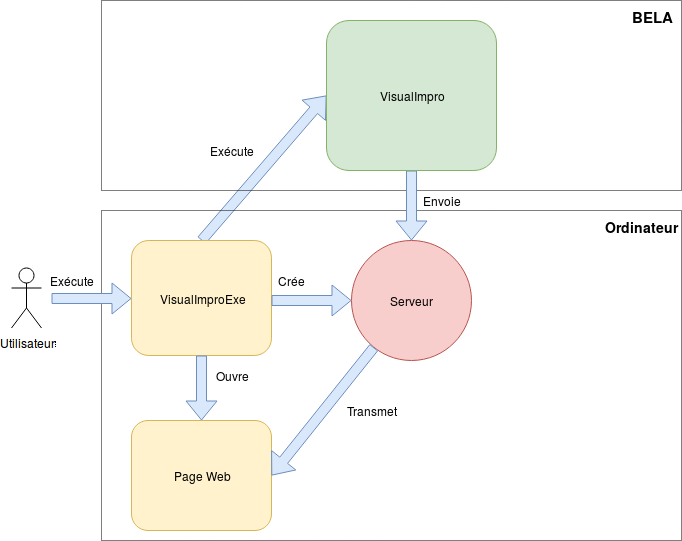
\includegraphics[scale=0.5]{assets/serveurGraph.png}
 \caption{architecture de base}
 \label{schéma global}
 
 
 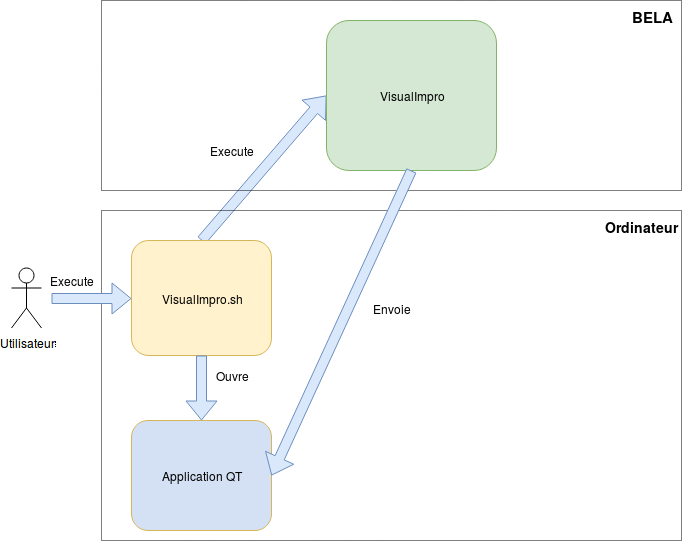
\includegraphics[scale=0.5]{assets/GUIRefeactored.png}
 \caption{Nouvelle architecture}
 \label{schéma global}
\end{figure}
\newpage

\paragraph{}
Le refactoring du code est également nécessaire au projet. En effet,
certains choix effectués par notre prédécesseur sur celui-ci nous
paraissent discutables. Notamment, le code est peu commenté, il est
parfois impossible de distinguer le code pré-existant dans Bela de
celui écrit par le programmeur, et le choix des outils destinés à
l'affichage de la matrice nous paraissent discutables. En effet,
Jérémy Lixandre ne semble pas justifier l'emploi de NodeJS et d'un
navigateur web pour l'affichage de la matrice graphique. Nous
choisissons alors de modifier ce processus d'affichage : la matrice
sera affichée via une simple interface graphique du framework Qt, ce
qui nous permet de rassembler l'ensemble du projet sous le langage
C++.
\paragraph{}
Le travail à effectuer sur le code existant se découpe alors en deux
parties : le refactoring du code d'une part, et l'implémentation du
retour sonore d'autre part.
